\chapter{Implementation}
\label{implementation}
\section{Introduction}
Following the design process, the two elements were designed separately and then integrated with Infandango. This step required understanding of how the Infandango system works, specifically how it renders webpages. The completed system gives a visual display for the predicted score retrieved from the model.

\section{Visual Design}
The final design is relatively simple and as the system is web based, web technologies like Javascript and CSS were considered. The choice between implementations strategies was based on the ease of integration with Infandango: although Infandango does already use Javascript like the Scriptaculous library\cite{scriptaculous_cite}, CSS is more heavily used. On the lab exercise page Infandango displays a single score for an exercise with a background colour determined by the score. Since this is already implemented using CSS, a similar approach was used for this implementation.

\section{Prediction Model}
The majority of the implementation for the model has already been performed when choosing the appropriate model: loading data, parsing data, training model and performing a prediction. The final remaining step is how to allow Infandango access to the model, a problem for which two solutions were created. 

When Infandango first starts, load the data and train the model. This object would then passed around to the appropriate place, staying in memory and being used whenever it is needed. A problem with this model is changing the model during runtime is more or less impossible without restarting Infandango. Another problem is that the data used for training would also need to be stored somewhere, which could require a separate database running alongside the active database. Finally, this could potentially cause some coupling between the code used for training the model and the Infandango startup procedure.

The second option is training the model before hand and storing/loading this model to be used when necessary. A problem with this approach is loading the model must occur during runtime which could potentially slow the loading speed of the web page. However, this approach does overcome some of the problem of the previous approach: the model can be changed easily, providing it uses the same loading interface; only the model needs to be stored, not all the data used for training; any model and training procedure can be used, as long as the same call can be made in order to make a prediction. The final implementation uses the training procedures discussed in chapter \ref{machinelearning} to train the model and serialises it using the standard python module, pickle.

\section{System Integration}
Infandango uses Django to generate the web pages. Django allows for the insertion of variables into HTML, which creates dynamic content. Each page has a method which generates the variables which can be used for that page. Since the progress bar is attaching to the sidebar - an item which appears on every page - then manually adding the prediction code to every page would take time and would be very difficult to change. Instead, Django offers "Context Processors" which is a way of hooking methods into the call to load any page, allowing these variables to be used by any page without telling every page explicitly. This also makes changing/removing the functionality much simpler. 




\section{Conclusion}
Using the Django context processor functionality a function is hooked into every web page request. This function de-serialises the trained model and uses it to provide a prediction based on previous exercise submissions. This prediction is used to determine the colours which will be displayed in each box and this is facilitated through Django. Figure \ref{fig:contextprocessor} shows how the control flow of this process.

\begin{figure}[h!]
\centering
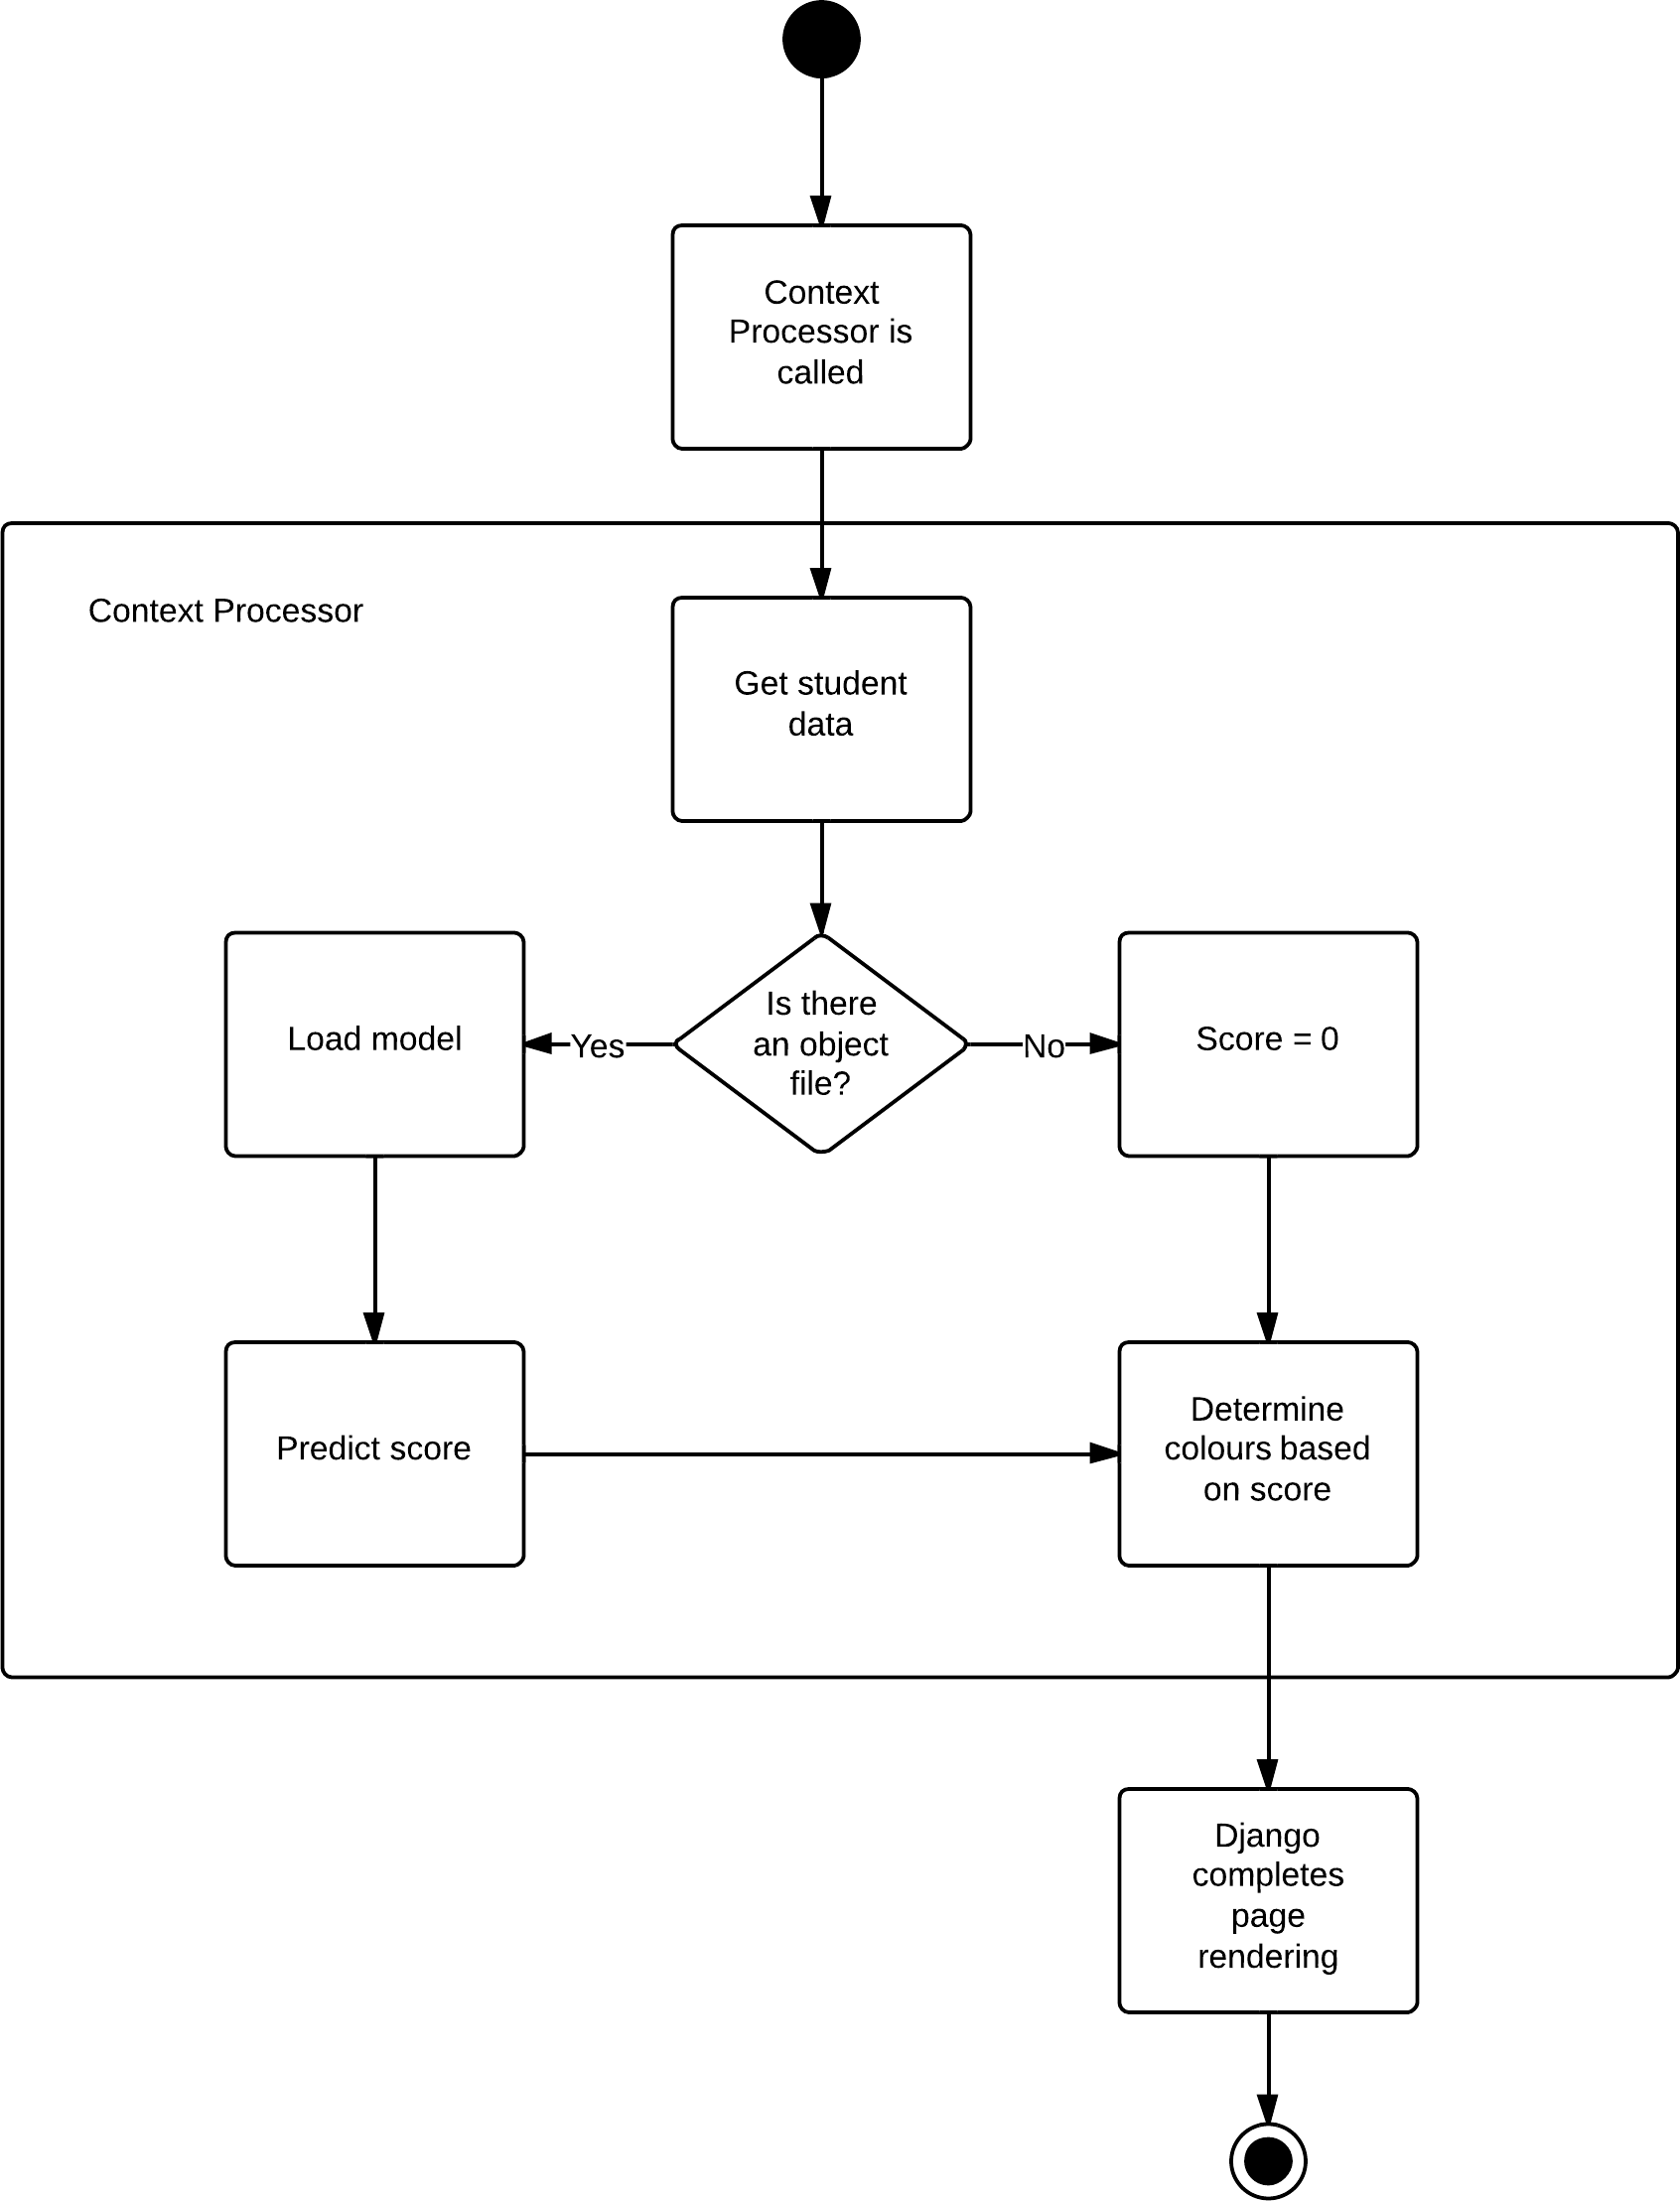
\includegraphics[width=0.8\textwidth]{images/contextprocessor.png}
\caption{A flowchart of the context processor function and how it interacts with Django}
\label{fig:contextprocessor}
\end{figure}
